\chapter{The Actor Model}
The actor model is a concurrency model, which first appeared in 1973 in the report "A Universal Modular ACTOR Formalism for Artificial Intelligence" by Carl Hewitt, Peter Bishop and Richard Steiger [worrydream.com/refs/Hewitt-ActorModel.pdf]. This chapter will explain the model generally. In addition to the general model, the model will be compared to alternative concurrency models and a few implementations of the model will be briefly described.

\section{Model}
The actor model is focused on the fact that any computational behaviour, be it functions, processes or data structures, can be modelled as a single behaviour; sending messages to actors.
An actor in this context is a process, which has its own isolated state, used to store values and modify its own behaviour, and a message box, for receiving messages. An actor can only share information by sending messages, asynchronously, to other actors. 
Actors are very similar to the communicating sequential processes (CSP) described in C.A.R. Hoare's publication "Communicating Sequential Processes". Actors, though, have a few well-defined behaviours in response to receiving a message, where CSPs are free to exhibit other behaviour. An actor can, in response to a message: 
\begin{enumerate}
  \item Send a finite number of messages to other actors.
  \item Spawn a finite number of new actors.
  \item Change its own behaviour for the next message that is received.
\end{enumerate}

In figure \ref{fig:actor}, a model of an actor based program can be seen.

\begin{figure}
  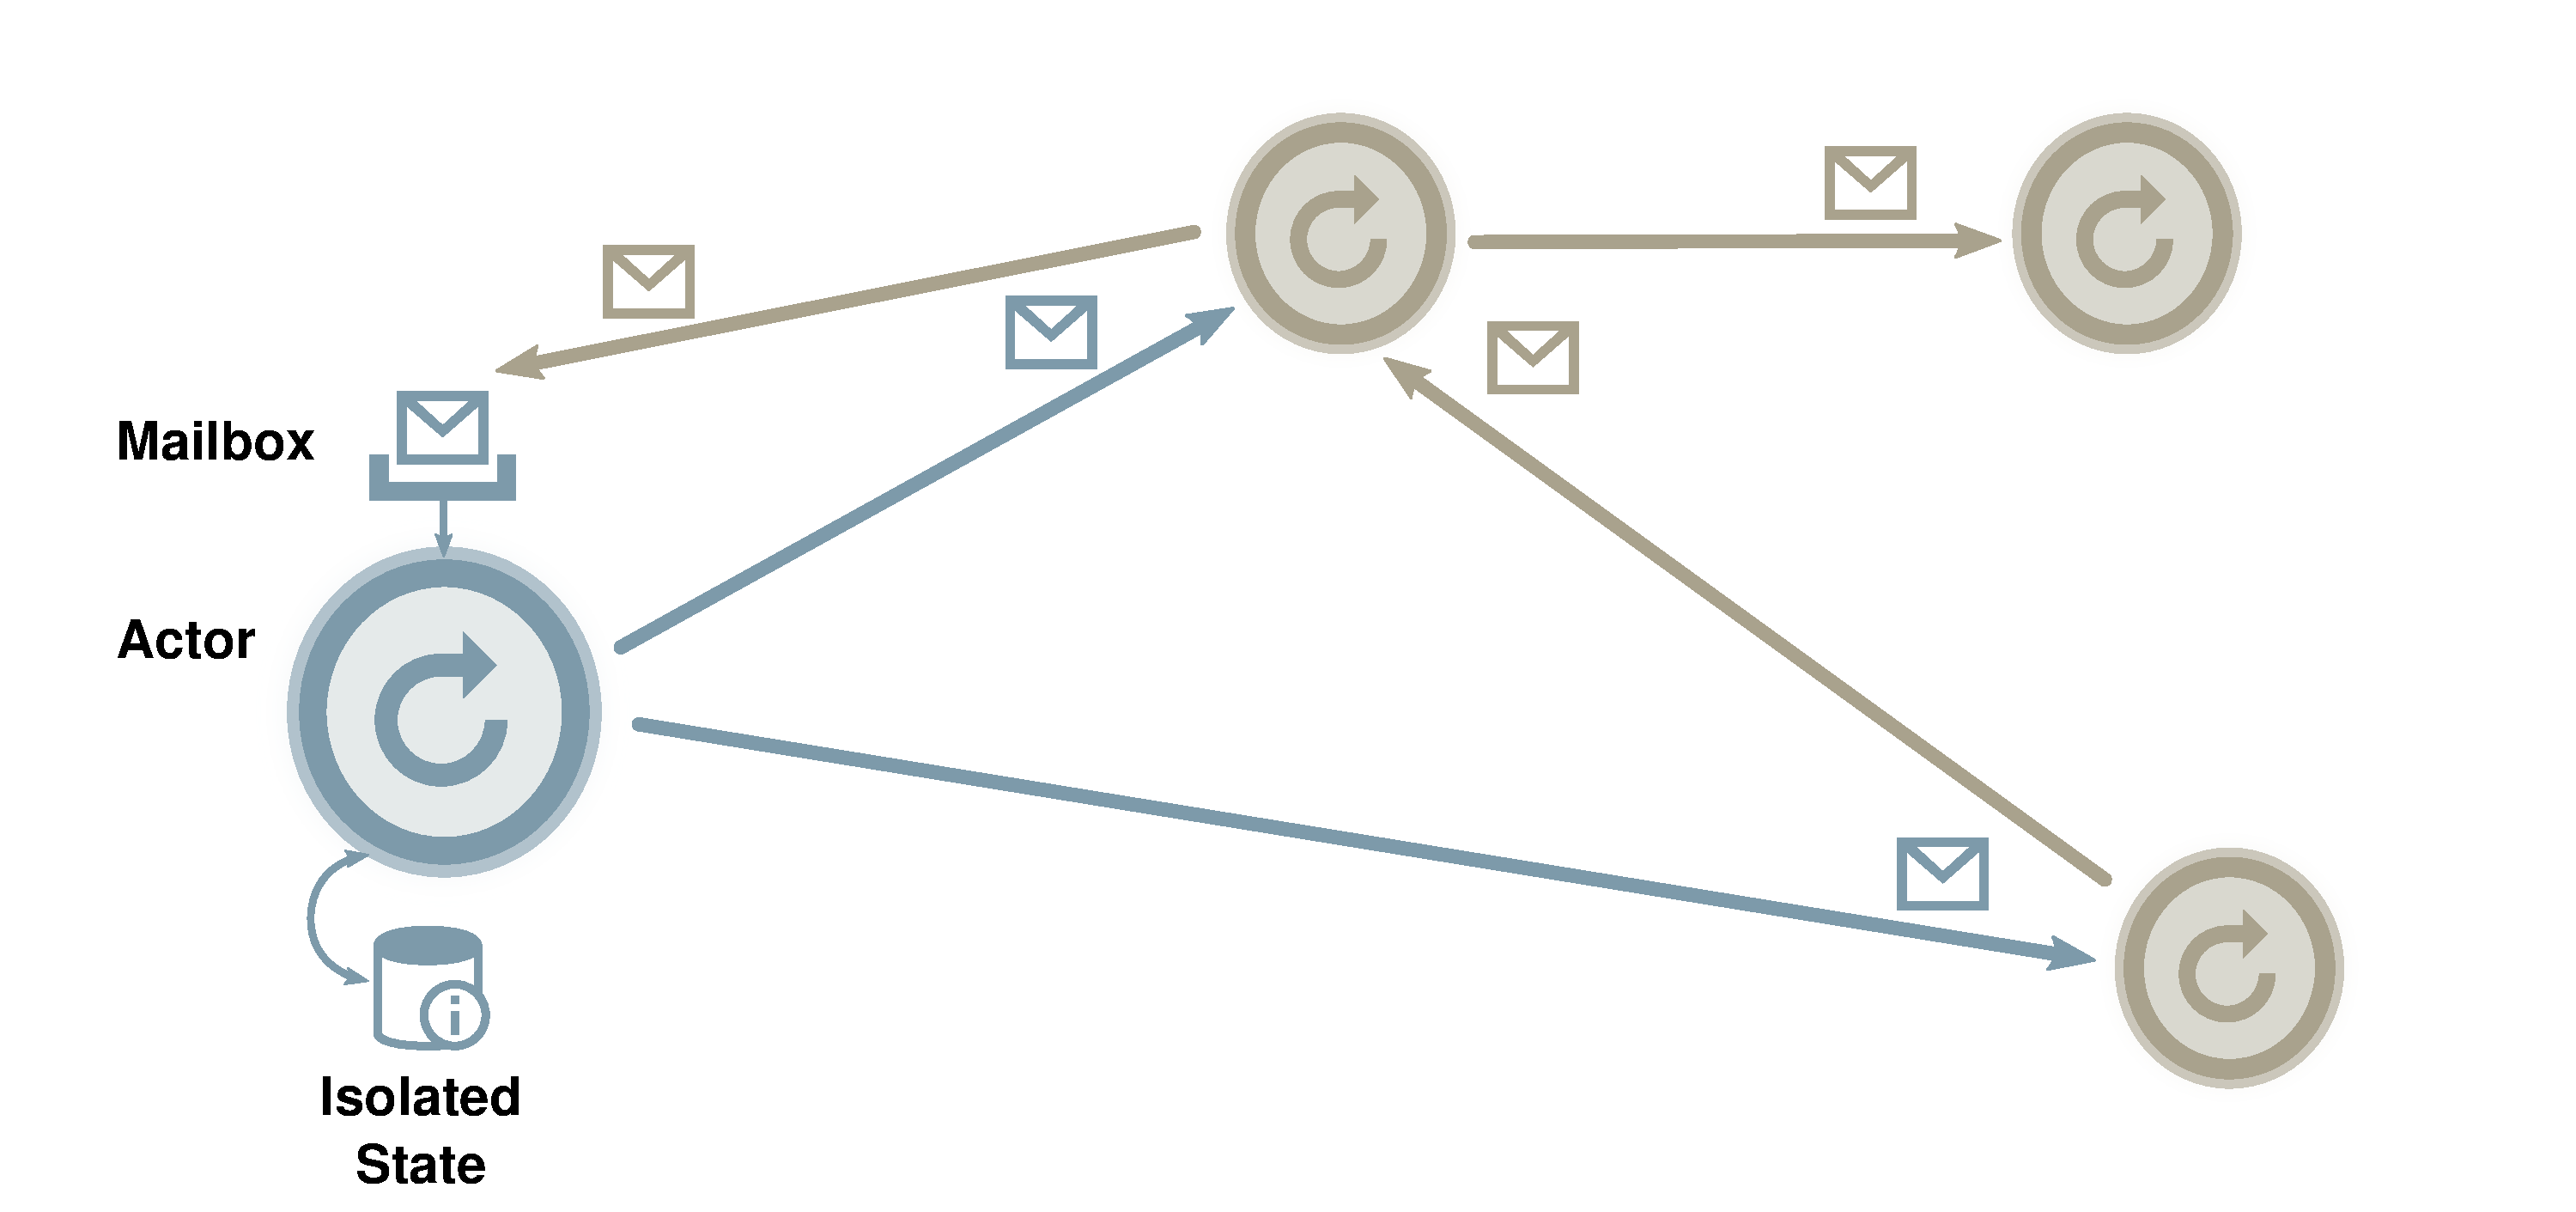
\includegraphics[width=\textwidth]{Images/actors.pdf}
  \caption{A model of an example program using actors. The nodes in this graph represent actors and the edges represent messages being sent.}
  \label{fig:actor}
\end{figure}


\subsection{Adding Logic}
One of the main features of the actor model is, as Hoare describes it, the ability to add knowledge to a system, without rewriting the existing knowledge. This means that if a developer is interested in adding a logical step in the business logic of his system, this can be achieved by merely adding an actor, which can perform the logical operations, that are to be added, and then adding that actor as a link in the flow of logic.

\subsubsection{Example}
We have a system which can read a CSV-file and print it to stdout. This can be implemented using actors in the following way:\\
let Reader and Printer be actors.

\begin{tabular}{ | c | c | c | }
\hline
Step & Reader & Printer \\\hline
1 & \textbf{Read CSV-file} & \textit{Wait for message} \\\hline
2 & \textbf{Send data to Printer} & \textit{Wait for message}\\\hline
3 & \textit{Wait for message} & \textbf{Receive data from Reader}\\\hline
4 & \textit{Wait for message} & \textbf{Print data to stdout}\\\hline
\end{tabular}\\
At som point we decide that we wish to format our data before printing it. To do so, we create and incorporate a new actor, Formatter, which changes the flow of execution in this manner:

\begin{tabular}{ | c | c | c | c | }
\hline
Step & Reader & Formatter & Printer \\\hline
1 & \textbf{Read CSV-file} & \textit{Wait for message} & \textit{Wait for message} \\\hline
2 & \textbf{Send data to Formatter} & \textit{Wait for message} & \textit{Wait for message}\\\hline
3 & \textit{Wait for message} & \textbf{Receive data} & \textit{Wait for message} \\\hline
4 & \textit{Wait for message} & \textbf{Format data} & \textit{Wait for message} \\\hline
5 & \textit{Wait for message} & \textbf{Send data to Printer} & \textit{Wait for message} \\\hline
6 & \textit{Wait for message} & \textit{Wait for message} & \textbf{Receive data}\\\hline
7 & \textit{Wait for message} & \textit{Wait for message} & \textbf{Print data to stdout} \\\hline
\end{tabular}\\

Notice that in adding the new logic, the only existing logic that was changed is the actor whom Reader sends data to.

\subsection{Supervisors}
Most implementations of the actor model implement a form of a supervisor-worker relationship. This means that every actor has a supervisor, typically their parent, to whom they report failures. The supervisor then has to deal with the failure, by for example restarting the failed actor.
Supervisors in the actor model works very well with the "fail fast"-principle of programming, meaning, in the actor model, that an actor will not try to continue operation or correct an error when encountering a failure. An actor that has failed will, as soon as the failure is detected, report the failure to its supervisor and halt operation, moving the responsibility of handling the failure up the supervision tree.

\section{Implementations}
\subsection{Erlang}
When talking about the actor model, one cannot escape the subject of Erlang. Erlang is one of first languages to fully incorporate the actor model as the main model of concurrency. Erlang is a purely functional language, developed for the telecommunications industry, where a lot of concurrent processes have to be handled. 
Actors in Erlang, or processes as they are called, are controlled by a few very simple constructs; actors can be spawned using the built-in spawn-function, the spawn-function takes three arguments, the module in which the actor is contained, the function that defines the behaviour for the actor and an initial message. You can send messages to actors using the bang-operator (!) and you can define an actor's behaviour in a receive-block.
In Erlang, an actor's parent is it's supervisor, if one chooses to use the supervisor module available. Using the supervisor module in Erlang gives the programmer the ability to choose different strategies to be used when a child actor fails. These strategies are:
\begin{enumerate}
  \item Respawn the failed child
  \item Respawn all children when one fails
  \item Respawn all children after the child in the start order of the children
\end{enumerate}

\subsubsection{Using actors in Erlang - Example}
To demonstrate the use of actors in Erlang, a simple example is shown in listing \ref{lst:ErlExample}. This program has only one actor, which counts the number of "incr"-messages it has been sent.

\begin{lstlisting}[style=erlang, caption={A simple message-counter in Erlang.}, label=lst:ErlExample]
-module(countMsgs).
-export([run/0, counter/1]).

run() ->
  S = spawn(countMsgs, counter, [0]), %spawn S as counter-actor
  sendMsgs(S, 10000), %send 10000 messages to S
  S.
  
counter(Sum) -> %function-definition for counter-actor
  receive
    value -> io:fwrite("Value is ~w~n", [Sum]);
    incr -> counter(Sum+1)
  end.

sendMsgs(_, 0) -> true; %base case
sendMsgs(S, N) -> %recursive function to send N messages to actor S
  S ! incr, %send incr to S
  sendMsgs(S, N-1).
\end{lstlisting}

\subsection{Akka}
A more modern approach to the actor model is taken in Akka, a concurrency toolkit for Scala and Java.
In Akka, an actor is just an object, which extends Akka's Actor-class and implements a receive method. One difference in the receive-method from Erlang's receive-block is that Akka's receive-method is exhaustive, meaning that the programmer has to define behaviour for all possible messages that an actor can receive. 
Creating an actor in Akka is done by calling the actorOf-method, on an actor or an instance of ActorSystem, which acts as the parent of top-level actors. The actorOf-method takes a Probs as an argument, Probs is just an object containing properties for an actor, such as the definition of the actor. Just like Erlang, messages are sent using the bang-operator.
In Akka, supervisors have the ability to handle failures in child actors in the following manner:
\begin{enumerate}
  \item Ignore failure and resume operation
  \item Restart the child from initial state
  \item Terminate the child, without respawning it
  \item Fail (move failure up supervision tree)
\end{enumerate}

\subsubsection{Using Actors in Akka - Example}
To demonstrate Akka's implementation of actors, the same example shown in listing \ref{lst:ErlExample} will be implemented in Scala, using Akka, in listing \ref{lst:AkkExample}.


\begin{lstlisting}[style = scala, caption={A simple message-counter in Scala.}, label=lst:AkkExample]

import akka.actor.Actor
import akka.actor.Probs

class Counter extends Actor{ //definition of counter-actor
  var count = 0
  def receive = {
    case "incr" => count += 1 //if actor receives "incr", increment count
    case "value" => println(s"Value is $count")
    case other => println(s"Error: Cannot understand message $other") //default case
  }
}

object Main extends App {
  val mySystem = ActorSystem("MySystem")
  val myCounter = mySystem.actorOf(Probs[Counter], name="MyCounter") //create counter-actor as top-level actor
  def main(args:Array[String]){
    for (i <- 1 to 10000) { //send 10000 messages to myCounter
      myCounter ! "incr"
    }
  }
}
\end{lstlisting}

